% Options for packages loaded elsewhere
\PassOptionsToPackage{unicode}{hyperref}
\PassOptionsToPackage{hyphens}{url}
\PassOptionsToPackage{dvipsnames,svgnames,x11names}{xcolor}
%
\documentclass[
  letterpaper,
  DIV=11,
  numbers=noendperiod]{scrartcl}

\usepackage{amsmath,amssymb}
\usepackage{iftex}
\ifPDFTeX
  \usepackage[T1]{fontenc}
  \usepackage[utf8]{inputenc}
  \usepackage{textcomp} % provide euro and other symbols
\else % if luatex or xetex
  \usepackage{unicode-math}
  \defaultfontfeatures{Scale=MatchLowercase}
  \defaultfontfeatures[\rmfamily]{Ligatures=TeX,Scale=1}
\fi
\usepackage{lmodern}
\ifPDFTeX\else  
    % xetex/luatex font selection
\fi
% Use upquote if available, for straight quotes in verbatim environments
\IfFileExists{upquote.sty}{\usepackage{upquote}}{}
\IfFileExists{microtype.sty}{% use microtype if available
  \usepackage[]{microtype}
  \UseMicrotypeSet[protrusion]{basicmath} % disable protrusion for tt fonts
}{}
\makeatletter
\@ifundefined{KOMAClassName}{% if non-KOMA class
  \IfFileExists{parskip.sty}{%
    \usepackage{parskip}
  }{% else
    \setlength{\parindent}{0pt}
    \setlength{\parskip}{6pt plus 2pt minus 1pt}}
}{% if KOMA class
  \KOMAoptions{parskip=half}}
\makeatother
\usepackage{xcolor}
\setlength{\emergencystretch}{3em} % prevent overfull lines
\setcounter{secnumdepth}{-\maxdimen} % remove section numbering
% Make \paragraph and \subparagraph free-standing
\makeatletter
\ifx\paragraph\undefined\else
  \let\oldparagraph\paragraph
  \renewcommand{\paragraph}{
    \@ifstar
      \xxxParagraphStar
      \xxxParagraphNoStar
  }
  \newcommand{\xxxParagraphStar}[1]{\oldparagraph*{#1}\mbox{}}
  \newcommand{\xxxParagraphNoStar}[1]{\oldparagraph{#1}\mbox{}}
\fi
\ifx\subparagraph\undefined\else
  \let\oldsubparagraph\subparagraph
  \renewcommand{\subparagraph}{
    \@ifstar
      \xxxSubParagraphStar
      \xxxSubParagraphNoStar
  }
  \newcommand{\xxxSubParagraphStar}[1]{\oldsubparagraph*{#1}\mbox{}}
  \newcommand{\xxxSubParagraphNoStar}[1]{\oldsubparagraph{#1}\mbox{}}
\fi
\makeatother

\usepackage{color}
\usepackage{fancyvrb}
\newcommand{\VerbBar}{|}
\newcommand{\VERB}{\Verb[commandchars=\\\{\}]}
\DefineVerbatimEnvironment{Highlighting}{Verbatim}{commandchars=\\\{\}}
% Add ',fontsize=\small' for more characters per line
\usepackage{framed}
\definecolor{shadecolor}{RGB}{241,243,245}
\newenvironment{Shaded}{\begin{snugshade}}{\end{snugshade}}
\newcommand{\AlertTok}[1]{\textcolor[rgb]{0.68,0.00,0.00}{#1}}
\newcommand{\AnnotationTok}[1]{\textcolor[rgb]{0.37,0.37,0.37}{#1}}
\newcommand{\AttributeTok}[1]{\textcolor[rgb]{0.40,0.45,0.13}{#1}}
\newcommand{\BaseNTok}[1]{\textcolor[rgb]{0.68,0.00,0.00}{#1}}
\newcommand{\BuiltInTok}[1]{\textcolor[rgb]{0.00,0.23,0.31}{#1}}
\newcommand{\CharTok}[1]{\textcolor[rgb]{0.13,0.47,0.30}{#1}}
\newcommand{\CommentTok}[1]{\textcolor[rgb]{0.37,0.37,0.37}{#1}}
\newcommand{\CommentVarTok}[1]{\textcolor[rgb]{0.37,0.37,0.37}{\textit{#1}}}
\newcommand{\ConstantTok}[1]{\textcolor[rgb]{0.56,0.35,0.01}{#1}}
\newcommand{\ControlFlowTok}[1]{\textcolor[rgb]{0.00,0.23,0.31}{\textbf{#1}}}
\newcommand{\DataTypeTok}[1]{\textcolor[rgb]{0.68,0.00,0.00}{#1}}
\newcommand{\DecValTok}[1]{\textcolor[rgb]{0.68,0.00,0.00}{#1}}
\newcommand{\DocumentationTok}[1]{\textcolor[rgb]{0.37,0.37,0.37}{\textit{#1}}}
\newcommand{\ErrorTok}[1]{\textcolor[rgb]{0.68,0.00,0.00}{#1}}
\newcommand{\ExtensionTok}[1]{\textcolor[rgb]{0.00,0.23,0.31}{#1}}
\newcommand{\FloatTok}[1]{\textcolor[rgb]{0.68,0.00,0.00}{#1}}
\newcommand{\FunctionTok}[1]{\textcolor[rgb]{0.28,0.35,0.67}{#1}}
\newcommand{\ImportTok}[1]{\textcolor[rgb]{0.00,0.46,0.62}{#1}}
\newcommand{\InformationTok}[1]{\textcolor[rgb]{0.37,0.37,0.37}{#1}}
\newcommand{\KeywordTok}[1]{\textcolor[rgb]{0.00,0.23,0.31}{\textbf{#1}}}
\newcommand{\NormalTok}[1]{\textcolor[rgb]{0.00,0.23,0.31}{#1}}
\newcommand{\OperatorTok}[1]{\textcolor[rgb]{0.37,0.37,0.37}{#1}}
\newcommand{\OtherTok}[1]{\textcolor[rgb]{0.00,0.23,0.31}{#1}}
\newcommand{\PreprocessorTok}[1]{\textcolor[rgb]{0.68,0.00,0.00}{#1}}
\newcommand{\RegionMarkerTok}[1]{\textcolor[rgb]{0.00,0.23,0.31}{#1}}
\newcommand{\SpecialCharTok}[1]{\textcolor[rgb]{0.37,0.37,0.37}{#1}}
\newcommand{\SpecialStringTok}[1]{\textcolor[rgb]{0.13,0.47,0.30}{#1}}
\newcommand{\StringTok}[1]{\textcolor[rgb]{0.13,0.47,0.30}{#1}}
\newcommand{\VariableTok}[1]{\textcolor[rgb]{0.07,0.07,0.07}{#1}}
\newcommand{\VerbatimStringTok}[1]{\textcolor[rgb]{0.13,0.47,0.30}{#1}}
\newcommand{\WarningTok}[1]{\textcolor[rgb]{0.37,0.37,0.37}{\textit{#1}}}

\providecommand{\tightlist}{%
  \setlength{\itemsep}{0pt}\setlength{\parskip}{0pt}}\usepackage{longtable,booktabs,array}
\usepackage{calc} % for calculating minipage widths
% Correct order of tables after \paragraph or \subparagraph
\usepackage{etoolbox}
\makeatletter
\patchcmd\longtable{\par}{\if@noskipsec\mbox{}\fi\par}{}{}
\makeatother
% Allow footnotes in longtable head/foot
\IfFileExists{footnotehyper.sty}{\usepackage{footnotehyper}}{\usepackage{footnote}}
\makesavenoteenv{longtable}
\usepackage{graphicx}
\makeatletter
\def\maxwidth{\ifdim\Gin@nat@width>\linewidth\linewidth\else\Gin@nat@width\fi}
\def\maxheight{\ifdim\Gin@nat@height>\textheight\textheight\else\Gin@nat@height\fi}
\makeatother
% Scale images if necessary, so that they will not overflow the page
% margins by default, and it is still possible to overwrite the defaults
% using explicit options in \includegraphics[width, height, ...]{}
\setkeys{Gin}{width=\maxwidth,height=\maxheight,keepaspectratio}
% Set default figure placement to htbp
\makeatletter
\def\fps@figure{htbp}
\makeatother

\KOMAoption{captions}{tableheading}
\makeatletter
\@ifpackageloaded{caption}{}{\usepackage{caption}}
\AtBeginDocument{%
\ifdefined\contentsname
  \renewcommand*\contentsname{Table of contents}
\else
  \newcommand\contentsname{Table of contents}
\fi
\ifdefined\listfigurename
  \renewcommand*\listfigurename{List of Figures}
\else
  \newcommand\listfigurename{List of Figures}
\fi
\ifdefined\listtablename
  \renewcommand*\listtablename{List of Tables}
\else
  \newcommand\listtablename{List of Tables}
\fi
\ifdefined\figurename
  \renewcommand*\figurename{Figure}
\else
  \newcommand\figurename{Figure}
\fi
\ifdefined\tablename
  \renewcommand*\tablename{Table}
\else
  \newcommand\tablename{Table}
\fi
}
\@ifpackageloaded{float}{}{\usepackage{float}}
\floatstyle{ruled}
\@ifundefined{c@chapter}{\newfloat{codelisting}{h}{lop}}{\newfloat{codelisting}{h}{lop}[chapter]}
\floatname{codelisting}{Listing}
\newcommand*\listoflistings{\listof{codelisting}{List of Listings}}
\makeatother
\makeatletter
\makeatother
\makeatletter
\@ifpackageloaded{caption}{}{\usepackage{caption}}
\@ifpackageloaded{subcaption}{}{\usepackage{subcaption}}
\makeatother

\ifLuaTeX
  \usepackage{selnolig}  % disable illegal ligatures
\fi
\usepackage{bookmark}

\IfFileExists{xurl.sty}{\usepackage{xurl}}{} % add URL line breaks if available
\urlstyle{same} % disable monospaced font for URLs
\hypersetup{
  pdftitle={Gradient Boosting Soccer Analysis},
  colorlinks=true,
  linkcolor={blue},
  filecolor={Maroon},
  citecolor={Blue},
  urlcolor={Blue},
  pdfcreator={LaTeX via pandoc}}


\title{Gradient Boosting Soccer Analysis}
\author{}
\date{}

\begin{document}
\maketitle


\begin{Shaded}
\begin{Highlighting}[]
\FunctionTok{library}\NormalTok{(caret)}
\end{Highlighting}
\end{Shaded}

\begin{verbatim}
Warning: package 'caret' was built under R version 4.3.3
\end{verbatim}

\begin{verbatim}
Loading required package: ggplot2
\end{verbatim}

\begin{verbatim}
Loading required package: lattice
\end{verbatim}

\begin{Shaded}
\begin{Highlighting}[]
\FunctionTok{library}\NormalTok{(lightgbm)}
\end{Highlighting}
\end{Shaded}

\begin{verbatim}
Warning: package 'lightgbm' was built under R version 4.3.3
\end{verbatim}

\begin{Shaded}
\begin{Highlighting}[]
\FunctionTok{library}\NormalTok{(ggplot2)}
\end{Highlighting}
\end{Shaded}

\begin{Shaded}
\begin{Highlighting}[]
\NormalTok{data }\OtherTok{\textless{}{-}} \FunctionTok{read.csv}\NormalTok{(}\StringTok{"transfer\_dataset.csv"}\NormalTok{)}
\NormalTok{cleaned\_data }\OtherTok{\textless{}{-}} \FunctionTok{na.omit}\NormalTok{(data)}
\end{Highlighting}
\end{Shaded}

\begin{Shaded}
\begin{Highlighting}[]
\FunctionTok{set.seed}\NormalTok{(}\DecValTok{278}\NormalTok{)}
\NormalTok{trainingIndex }\OtherTok{\textless{}{-}} \FunctionTok{createDataPartition}\NormalTok{(cleaned\_data}\SpecialCharTok{$}\NormalTok{transfer, }\AttributeTok{p =} \FloatTok{0.8}\NormalTok{, }\AttributeTok{list =} \ConstantTok{FALSE}\NormalTok{)}
\NormalTok{train\_data }\OtherTok{\textless{}{-}}\NormalTok{ cleaned\_data[trainingIndex,]}
\NormalTok{test\_data }\OtherTok{\textless{}{-}}\NormalTok{ cleaned\_data[}\SpecialCharTok{{-}}\NormalTok{trainingIndex, ]}
\NormalTok{train\_data }\OtherTok{\textless{}{-}}\NormalTok{ train\_data[, }\FunctionTok{setdiff}\NormalTok{(}\FunctionTok{names}\NormalTok{(train\_data), }\StringTok{"name"}\NormalTok{)]}
\NormalTok{test\_data }\OtherTok{\textless{}{-}}\NormalTok{ test\_data[, }\FunctionTok{setdiff}\NormalTok{(}\FunctionTok{names}\NormalTok{(test\_data), }\StringTok{"name"}\NormalTok{)]}
\end{Highlighting}
\end{Shaded}

\begin{Shaded}
\begin{Highlighting}[]
\NormalTok{lgbtrain }\OtherTok{\textless{}{-}} \FunctionTok{lgb.Dataset}\NormalTok{(}\AttributeTok{data =} \FunctionTok{as.matrix}\NormalTok{(train\_data[, }\FunctionTok{setdiff}\NormalTok{(}\FunctionTok{names}\NormalTok{(train\_data), }\StringTok{"transfer"}\NormalTok{)]), }\AttributeTok{label =}\NormalTok{ train\_data}\SpecialCharTok{$}\NormalTok{transfer)}
\end{Highlighting}
\end{Shaded}

\begin{verbatim}
Warning in storage.mode(data) <- "double": NAs introduced by coercion
\end{verbatim}

\begin{Shaded}
\begin{Highlighting}[]
\NormalTok{lgbtest }\OtherTok{\textless{}{-}} \FunctionTok{lgb.Dataset}\NormalTok{(}\AttributeTok{data =} \FunctionTok{as.matrix}\NormalTok{(test\_data[, }\FunctionTok{setdiff}\NormalTok{(}\FunctionTok{names}\NormalTok{(test\_data), }\StringTok{"transfer"}\NormalTok{)]), }\AttributeTok{label =}\NormalTok{ test\_data}\SpecialCharTok{$}\NormalTok{transfer)}
\end{Highlighting}
\end{Shaded}

\begin{verbatim}
Warning in storage.mode(data) <- "double": NAs introduced by coercion
\end{verbatim}

\begin{Shaded}
\begin{Highlighting}[]
\NormalTok{parameters }\OtherTok{\textless{}{-}} \FunctionTok{list}\NormalTok{(}
  \AttributeTok{objective =} \StringTok{"binary"}\NormalTok{,}
  \AttributeTok{boosting\_type =} \StringTok{"gbdt"}\NormalTok{,}
  \AttributeTok{learning\_rate =} \FloatTok{0.05}\NormalTok{,}
  \AttributeTok{num\_leaves =} \DecValTok{75}
\NormalTok{)}
\end{Highlighting}
\end{Shaded}

\begin{Shaded}
\begin{Highlighting}[]
\NormalTok{gbm\_model }\OtherTok{\textless{}{-}} \FunctionTok{lgb.train}\NormalTok{(}
  \AttributeTok{params =}\NormalTok{ parameters,}
  \AttributeTok{data =}\NormalTok{ lgbtrain,}
  \AttributeTok{nrounds =} \DecValTok{100}\NormalTok{,}
  \AttributeTok{valids =} \FunctionTok{list}\NormalTok{(}\AttributeTok{test =}\NormalTok{ lgbtest),}
  \AttributeTok{early\_stopping\_rounds =} \DecValTok{10}
\NormalTok{)}
\end{Highlighting}
\end{Shaded}

\begin{verbatim}
[LightGBM] [Info] Number of positive: 208, number of negative: 3092
[LightGBM] [Info] Auto-choosing row-wise multi-threading, the overhead of testing was 0.001553 seconds.
You can set `force_row_wise=true` to remove the overhead.
And if memory is not enough, you can set `force_col_wise=true`.
[LightGBM] [Info] Total Bins 3622
[LightGBM] [Info] Number of data points in the train set: 3300, number of used features: 29
[LightGBM] [Info] [binary:BoostFromScore]: pavg=0.063030 -> initscore=-2.699035
[LightGBM] [Info] Start training from score -2.699035
[1]:  test's binary_logloss:0.214395 
Will train until there is no improvement in 10 rounds.
[2]:  test's binary_logloss:0.213645 
[3]:  test's binary_logloss:0.211696 
[4]:  test's binary_logloss:0.211212 
[5]:  test's binary_logloss:0.210115 
[6]:  test's binary_logloss:0.210085 
[7]:  test's binary_logloss:0.209526 
[8]:  test's binary_logloss:0.20989 
[9]:  test's binary_logloss:0.210281 
[10]:  test's binary_logloss:0.210762 
[11]:  test's binary_logloss:0.210959 
[12]:  test's binary_logloss:0.210799 
[13]:  test's binary_logloss:0.210601 
[14]:  test's binary_logloss:0.210762 
[15]:  test's binary_logloss:0.211527 
[16]:  test's binary_logloss:0.212129 
[17]:  test's binary_logloss:0.211673 
Early stopping, best iteration is: [7]:  test's binary_logloss:0.209526
\end{verbatim}

\begin{Shaded}
\begin{Highlighting}[]
\NormalTok{predictions }\OtherTok{\textless{}{-}} \FunctionTok{predict}\NormalTok{(gbm\_model,}
                       \FunctionTok{as.matrix}\NormalTok{(test\_data[,}\FunctionTok{setdiff}\NormalTok{(}\FunctionTok{names}\NormalTok{(test\_data),}
                                                    \StringTok{"transfer"}\NormalTok{)]), }\AttributeTok{label =}
\NormalTok{                         test\_data}\SpecialCharTok{$}\NormalTok{transfer)}
\end{Highlighting}
\end{Shaded}

\begin{verbatim}
Warning in predict.lgb.Booster(gbm_model, as.matrix(test_data[,
setdiff(names(test_data), : predict.lgb.Booster: Found the following passed
through '...': label. These are ignored. Use argument 'params' instead.
\end{verbatim}

\begin{verbatim}
Warning in storage.mode(data) <- "double": NAs introduced by coercion
\end{verbatim}

\begin{Shaded}
\begin{Highlighting}[]
\FunctionTok{summary}\NormalTok{(predictions)}
\end{Highlighting}
\end{Shaded}

\begin{verbatim}
   Min. 1st Qu.  Median    Mean 3rd Qu.    Max. 
0.04420 0.04808 0.05690 0.06430 0.07204 0.23672 
\end{verbatim}

\begin{Shaded}
\begin{Highlighting}[]
\NormalTok{binary\_predictions }\OtherTok{\textless{}{-}} \FunctionTok{ifelse}\NormalTok{(predictions }\SpecialCharTok{\textgreater{}} \FloatTok{0.5}\NormalTok{, }\DecValTok{1}\NormalTok{, }\DecValTok{0}\NormalTok{)}

\NormalTok{accuracy }\OtherTok{\textless{}{-}} \FunctionTok{mean}\NormalTok{(binary\_predictions }\SpecialCharTok{==}\NormalTok{ test\_data}\SpecialCharTok{$}\NormalTok{transfer)}
\FunctionTok{cat}\NormalTok{(}\StringTok{"Accuracy:"}\NormalTok{, accuracy, }\StringTok{"}\SpecialCharTok{\textbackslash{}n}\StringTok{"}\NormalTok{)}
\end{Highlighting}
\end{Shaded}

\begin{verbatim}
Accuracy: 0.9441748 
\end{verbatim}

Model Statistics

\begin{Shaded}
\begin{Highlighting}[]
\ControlFlowTok{if}\NormalTok{ (}\SpecialCharTok{!}\FunctionTok{require}\NormalTok{(knitr)) }\FunctionTok{install.packages}\NormalTok{(}\StringTok{"knitr"}\NormalTok{)}
\end{Highlighting}
\end{Shaded}

\begin{verbatim}
Loading required package: knitr
\end{verbatim}

\begin{Shaded}
\begin{Highlighting}[]
\FunctionTok{library}\NormalTok{(knitr)}

\CommentTok{\# Binary predictions from the model}
\NormalTok{binary\_predictions }\OtherTok{\textless{}{-}} \FunctionTok{ifelse}\NormalTok{(predictions }\SpecialCharTok{\textgreater{}} \FloatTok{0.5}\NormalTok{, }\DecValTok{1}\NormalTok{, }\DecValTok{0}\NormalTok{)}

\CommentTok{\# Compute confusion matrix}
\NormalTok{conf\_matrix }\OtherTok{\textless{}{-}} \FunctionTok{confusionMatrix}\NormalTok{(}\FunctionTok{factor}\NormalTok{(binary\_predictions),}
                               \FunctionTok{factor}\NormalTok{(test\_data}\SpecialCharTok{$}\NormalTok{transfer))}
\end{Highlighting}
\end{Shaded}

\begin{verbatim}
Warning in confusionMatrix.default(factor(binary_predictions),
factor(test_data$transfer)): Levels are not in the same order for reference and
data. Refactoring data to match.
\end{verbatim}

\begin{Shaded}
\begin{Highlighting}[]
\CommentTok{\# Extract relevant metrics}
\NormalTok{accuracy }\OtherTok{\textless{}{-}}\NormalTok{ conf\_matrix}\SpecialCharTok{$}\NormalTok{overall[}\StringTok{"Accuracy"}\NormalTok{]}
\NormalTok{precision }\OtherTok{\textless{}{-}}\NormalTok{ conf\_matrix}\SpecialCharTok{$}\NormalTok{byClass[}\StringTok{"Precision"}\NormalTok{]}
\NormalTok{recall }\OtherTok{\textless{}{-}}\NormalTok{ conf\_matrix}\SpecialCharTok{$}\NormalTok{byClass[}\StringTok{"Recall"}\NormalTok{]}
\NormalTok{f1\_score }\OtherTok{\textless{}{-}}\NormalTok{ conf\_matrix}\SpecialCharTok{$}\NormalTok{byClass[}\StringTok{"F1"}\NormalTok{]}
\NormalTok{kappa }\OtherTok{\textless{}{-}}\NormalTok{ conf\_matrix}\SpecialCharTok{$}\NormalTok{overall[}\StringTok{"Kappa"}\NormalTok{]}

\CommentTok{\# Create a data frame for the metrics}
\NormalTok{metrics\_df }\OtherTok{\textless{}{-}} \FunctionTok{data.frame}\NormalTok{(}
  \AttributeTok{Metric =} \FunctionTok{c}\NormalTok{(}\StringTok{"Accuracy"}\NormalTok{, }\StringTok{"Precision"}\NormalTok{, }\StringTok{"Recall"}\NormalTok{, }\StringTok{"F1{-}Score"}\NormalTok{, }\StringTok{"Kappa"}\NormalTok{),}
  \AttributeTok{Value =} \FunctionTok{c}\NormalTok{(accuracy, precision, recall, f1\_score, kappa)}
\NormalTok{)}

\CommentTok{\# Use kable to create a formatted table}
\FunctionTok{kable}\NormalTok{(metrics\_df, }\AttributeTok{col.names =} \FunctionTok{c}\NormalTok{(}\StringTok{"Metric"}\NormalTok{, }\StringTok{"Value"}\NormalTok{), }\AttributeTok{caption =} \StringTok{"Model Evaluation Metrics"}\NormalTok{)}
\end{Highlighting}
\end{Shaded}

\begin{longtable}[]{@{}llr@{}}
\caption{Model Evaluation Metrics}\tabularnewline
\toprule\noalign{}
& Metric & Value \\
\midrule\noalign{}
\endfirsthead
\toprule\noalign{}
& Metric & Value \\
\midrule\noalign{}
\endhead
\bottomrule\noalign{}
\endlastfoot
Accuracy & Accuracy & 0.9441748 \\
Precision & Precision & 0.9441748 \\
Recall & Recall & 1.0000000 \\
F1 & F1-Score & 0.9712859 \\
Kappa & Kappa & 0.0000000 \\
\end{longtable}

Visualization

\begin{Shaded}
\begin{Highlighting}[]
\FunctionTok{library}\NormalTok{(pROC)}
\end{Highlighting}
\end{Shaded}

\begin{verbatim}
Warning: package 'pROC' was built under R version 4.3.3
\end{verbatim}

\begin{verbatim}
Type 'citation("pROC")' for a citation.
\end{verbatim}

\begin{verbatim}

Attaching package: 'pROC'
\end{verbatim}

\begin{verbatim}
The following objects are masked from 'package:stats':

    cov, smooth, var
\end{verbatim}

\begin{Shaded}
\begin{Highlighting}[]
\NormalTok{roc\_obj }\OtherTok{\textless{}{-}} \FunctionTok{roc}\NormalTok{(test\_data}\SpecialCharTok{$}\NormalTok{transfer, predictions)}
\end{Highlighting}
\end{Shaded}

\begin{verbatim}
Setting levels: control = 0, case = 1
\end{verbatim}

\begin{verbatim}
Setting direction: controls < cases
\end{verbatim}

\begin{Shaded}
\begin{Highlighting}[]
\NormalTok{roc\_data }\OtherTok{\textless{}{-}} \FunctionTok{data.frame}\NormalTok{(}\AttributeTok{TPR =}\NormalTok{ roc\_obj}\SpecialCharTok{$}\NormalTok{sensitivities,}
  \AttributeTok{FPR =} \DecValTok{1} \SpecialCharTok{{-}}\NormalTok{ roc\_obj}\SpecialCharTok{$}\NormalTok{specificities,}
  \AttributeTok{Thresholds =}\NormalTok{ roc\_obj}\SpecialCharTok{$}\NormalTok{thresholds}
\NormalTok{)}
\NormalTok{roc\_g }\OtherTok{\textless{}{-}} \FunctionTok{ggplot}\NormalTok{(roc\_data, }\FunctionTok{aes}\NormalTok{(}\AttributeTok{x =}\NormalTok{ FPR, }\AttributeTok{y =}\NormalTok{ TPR)) }\SpecialCharTok{+}
  \FunctionTok{geom\_line}\NormalTok{(}\AttributeTok{color =} \StringTok{"blue"}\NormalTok{) }\SpecialCharTok{+} 
  \FunctionTok{geom\_abline}\NormalTok{(}\AttributeTok{slope =} \DecValTok{1}\NormalTok{, }\AttributeTok{intercept =} \DecValTok{0}\NormalTok{, }\AttributeTok{linetype =} \StringTok{"dashed"}\NormalTok{, }\AttributeTok{color =} \StringTok{"red"}\NormalTok{) }\SpecialCharTok{+}
  \FunctionTok{labs}\NormalTok{(}\AttributeTok{title =} \StringTok{"ROC Curve"}\NormalTok{, }\AttributeTok{x =} \StringTok{"False Positive Rate"}\NormalTok{, }\AttributeTok{y =} \StringTok{"True Positive Rate"}\NormalTok{) }\SpecialCharTok{+}
  \FunctionTok{theme\_minimal}\NormalTok{()}

\NormalTok{roc\_g}
\end{Highlighting}
\end{Shaded}

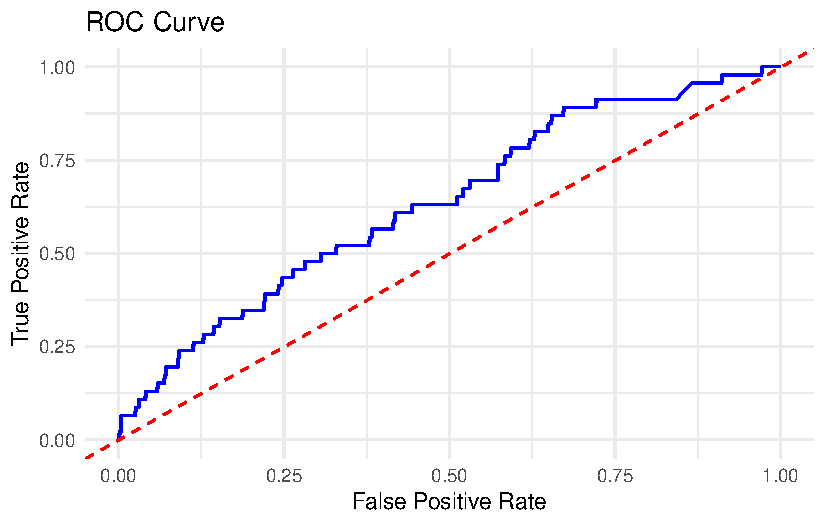
\includegraphics{aaron_lightGBM_modeling_files/figure-pdf/unnamed-chunk-10-1.pdf}

Precision-Recall Curve

\begin{Shaded}
\begin{Highlighting}[]
\CommentTok{\# Calculate Precision and Recall}
\NormalTok{thresholds }\OtherTok{\textless{}{-}} \FunctionTok{seq}\NormalTok{(}\DecValTok{0}\NormalTok{, }\DecValTok{1}\NormalTok{, }\AttributeTok{by =} \FloatTok{0.01}\NormalTok{)}
\NormalTok{precision }\OtherTok{\textless{}{-}} \FunctionTok{sapply}\NormalTok{(thresholds, }\ControlFlowTok{function}\NormalTok{(thresh) \{}
\NormalTok{  predicted\_labels }\OtherTok{\textless{}{-}} \FunctionTok{ifelse}\NormalTok{(predictions }\SpecialCharTok{\textgreater{}}\NormalTok{ thresh, }\DecValTok{1}\NormalTok{, }\DecValTok{0}\NormalTok{)}
  \FunctionTok{sum}\NormalTok{(predicted\_labels }\SpecialCharTok{\&}\NormalTok{ test\_data}\SpecialCharTok{$}\NormalTok{transfer) }\SpecialCharTok{/} \FunctionTok{sum}\NormalTok{(predicted\_labels)}
\NormalTok{\})}
\NormalTok{recall }\OtherTok{\textless{}{-}} \FunctionTok{sapply}\NormalTok{(thresholds, }\ControlFlowTok{function}\NormalTok{(thresh) \{}
\NormalTok{  predicted\_labels }\OtherTok{\textless{}{-}} \FunctionTok{ifelse}\NormalTok{(predictions }\SpecialCharTok{\textgreater{}}\NormalTok{ thresh, }\DecValTok{1}\NormalTok{, }\DecValTok{0}\NormalTok{)}
  \FunctionTok{sum}\NormalTok{(predicted\_labels }\SpecialCharTok{\&}\NormalTok{ test\_data}\SpecialCharTok{$}\NormalTok{transfer) }\SpecialCharTok{/} \FunctionTok{sum}\NormalTok{(test\_data}\SpecialCharTok{$}\NormalTok{transfer)}
\NormalTok{\})}

\CommentTok{\# Plot Precision{-}Recall Curve}
\NormalTok{pr\_curve\_g }\OtherTok{\textless{}{-}} \FunctionTok{plot}\NormalTok{(recall, precision, }\AttributeTok{type =} \StringTok{"l"}\NormalTok{, }\AttributeTok{col =} \StringTok{"red"}\NormalTok{, }\AttributeTok{main =} \StringTok{"Precision{-}Recall Curve"}\NormalTok{,}
     \AttributeTok{xlim =} \FunctionTok{c}\NormalTok{(}\DecValTok{0}\NormalTok{,}\DecValTok{1}\NormalTok{), }\AttributeTok{ylim =} \FunctionTok{c}\NormalTok{(}\DecValTok{0}\NormalTok{,}\DecValTok{1}\NormalTok{), }\AttributeTok{xlab =} \StringTok{"Recall"}\NormalTok{, }\AttributeTok{ylab =} \StringTok{"Precision"}\NormalTok{)}
\end{Highlighting}
\end{Shaded}

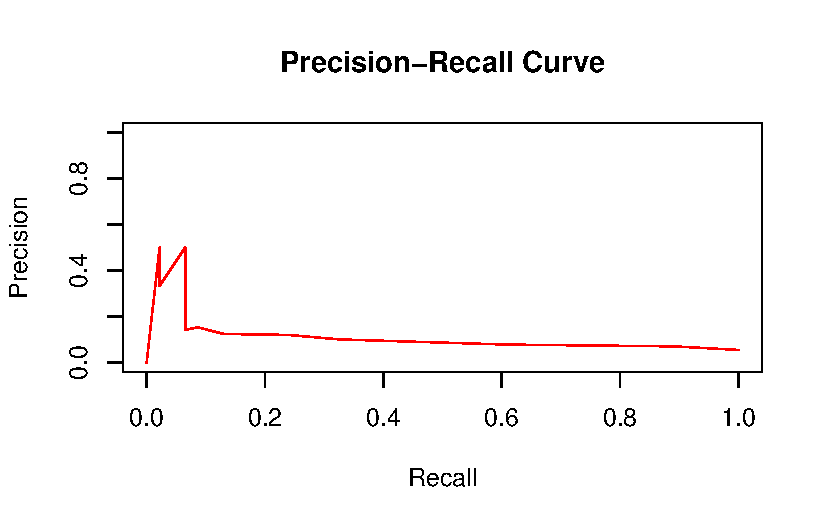
\includegraphics{aaron_lightGBM_modeling_files/figure-pdf/unnamed-chunk-11-1.pdf}

\begin{Shaded}
\begin{Highlighting}[]
\CommentTok{\# Create Confusion Matrix}
\NormalTok{binary\_predictions }\OtherTok{\textless{}{-}} \FunctionTok{ifelse}\NormalTok{(predictions }\SpecialCharTok{\textgreater{}} \FloatTok{0.5}\NormalTok{, }\DecValTok{1}\NormalTok{, }\DecValTok{0}\NormalTok{)}
\NormalTok{conf\_matrix }\OtherTok{\textless{}{-}} \FunctionTok{confusionMatrix}\NormalTok{(}\FunctionTok{factor}\NormalTok{(binary\_predictions),}
                               \FunctionTok{factor}\NormalTok{(test\_data}\SpecialCharTok{$}\NormalTok{transfer))}
\end{Highlighting}
\end{Shaded}

\begin{verbatim}
Warning in confusionMatrix.default(factor(binary_predictions),
factor(test_data$transfer)): Levels are not in the same order for reference and
data. Refactoring data to match.
\end{verbatim}

\begin{Shaded}
\begin{Highlighting}[]
\CommentTok{\# Plot Confusion Matrix}
\FunctionTok{library}\NormalTok{(ggplot2)}
\NormalTok{conf\_df }\OtherTok{\textless{}{-}} \FunctionTok{as.data.frame}\NormalTok{(conf\_matrix}\SpecialCharTok{$}\NormalTok{table)}
\NormalTok{conf\_df}\SpecialCharTok{$}\NormalTok{Prediction }\OtherTok{\textless{}{-}} \FunctionTok{factor}\NormalTok{(conf\_df}\SpecialCharTok{$}\NormalTok{Prediction, }\AttributeTok{levels =} \FunctionTok{c}\NormalTok{(}\DecValTok{0}\NormalTok{, }\DecValTok{1}\NormalTok{),}
                             \AttributeTok{labels =} \FunctionTok{c}\NormalTok{(}\StringTok{"no transfer"}\NormalTok{, }\StringTok{"transferred"}\NormalTok{))}
\NormalTok{conf\_df}\SpecialCharTok{$}\NormalTok{Reference }\OtherTok{\textless{}{-}} \FunctionTok{factor}\NormalTok{(conf\_df}\SpecialCharTok{$}\NormalTok{Reference, }\AttributeTok{levels =} \FunctionTok{c}\NormalTok{(}\DecValTok{0}\NormalTok{,}\DecValTok{1}\NormalTok{),}
                            \AttributeTok{labels =} \FunctionTok{c}\NormalTok{(}\StringTok{"no transfer"}\NormalTok{, }\StringTok{"tranferred"}\NormalTok{))}
\NormalTok{conf\_matrix\_g }\OtherTok{\textless{}{-}} \FunctionTok{ggplot}\NormalTok{(}\AttributeTok{data =}\NormalTok{ conf\_df, }\FunctionTok{aes}\NormalTok{(}\AttributeTok{x =}\NormalTok{ Reference, }\AttributeTok{y =}\NormalTok{ Prediction)) }\SpecialCharTok{+}
  \FunctionTok{geom\_tile}\NormalTok{(}\FunctionTok{aes}\NormalTok{(}\AttributeTok{fill =}\NormalTok{ Freq), }\AttributeTok{color =} \StringTok{"white"}\NormalTok{) }\SpecialCharTok{+}
  \FunctionTok{scale\_fill\_gradient}\NormalTok{(}\AttributeTok{low =} \StringTok{"blue"}\NormalTok{, }\AttributeTok{high =} \StringTok{"red"}\NormalTok{) }\SpecialCharTok{+}
  \FunctionTok{geom\_text}\NormalTok{(}\FunctionTok{aes}\NormalTok{(}\AttributeTok{label =}\NormalTok{ Freq)) }\SpecialCharTok{+}
  \FunctionTok{theme\_minimal}\NormalTok{() }\SpecialCharTok{+}
  \FunctionTok{labs}\NormalTok{(}\AttributeTok{title =} \StringTok{"LightGbm Confusion Matrix"}\NormalTok{, }\AttributeTok{fill =} \StringTok{"Frequency"}\NormalTok{,}
       \AttributeTok{x =} \StringTok{"Actual Status"}\NormalTok{, }\AttributeTok{y =} \StringTok{"Predicted Status"}\NormalTok{)}

\NormalTok{conf\_matrix\_g}
\end{Highlighting}
\end{Shaded}

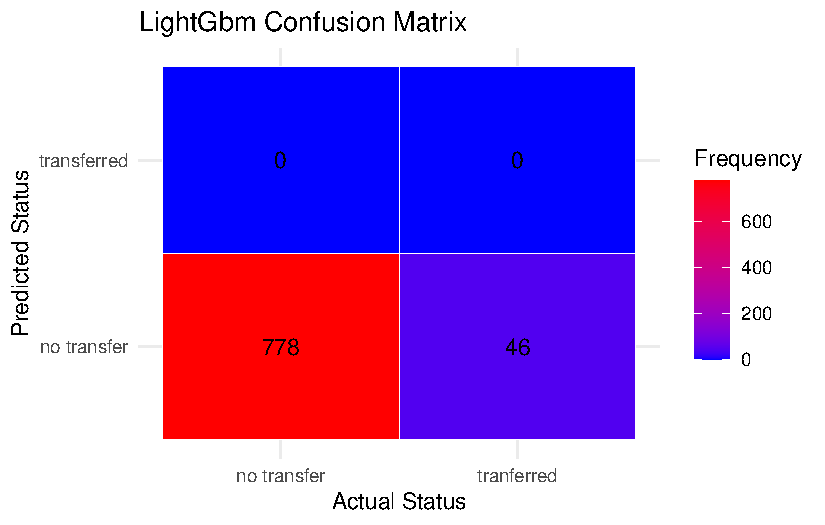
\includegraphics{aaron_lightGBM_modeling_files/figure-pdf/unnamed-chunk-12-1.pdf}

\begin{Shaded}
\begin{Highlighting}[]
\NormalTok{importance }\OtherTok{\textless{}{-}} \FunctionTok{lgb.importance}\NormalTok{(gbm\_model)}
\NormalTok{importance\_df }\OtherTok{\textless{}{-}} \FunctionTok{as.data.frame}\NormalTok{(importance)}

\NormalTok{variable\_importance\_g }\OtherTok{\textless{}{-}} \FunctionTok{ggplot}\NormalTok{(importance\_df, }\FunctionTok{aes}\NormalTok{(}\AttributeTok{x =} \FunctionTok{reorder}\NormalTok{(Feature, Gain),}
                                                   \AttributeTok{y =}\NormalTok{ Gain)) }\SpecialCharTok{+}
  \FunctionTok{geom\_bar}\NormalTok{(}\AttributeTok{stat =} \StringTok{"identity"}\NormalTok{, }\AttributeTok{fill =} \StringTok{"skyblue"}\NormalTok{) }\SpecialCharTok{+}
  \FunctionTok{coord\_flip}\NormalTok{() }\SpecialCharTok{+}
  \FunctionTok{theme\_minimal}\NormalTok{() }\SpecialCharTok{+}
  \FunctionTok{labs}\NormalTok{(}\AttributeTok{title =} \StringTok{"Feature Importance"}\NormalTok{, }\AttributeTok{x =} \StringTok{"Feature"}\NormalTok{,}
       \AttributeTok{y =} \StringTok{"Gain (Improvement in Log Loss When Splitting)"}\NormalTok{)}

\NormalTok{variable\_importance\_g}
\end{Highlighting}
\end{Shaded}

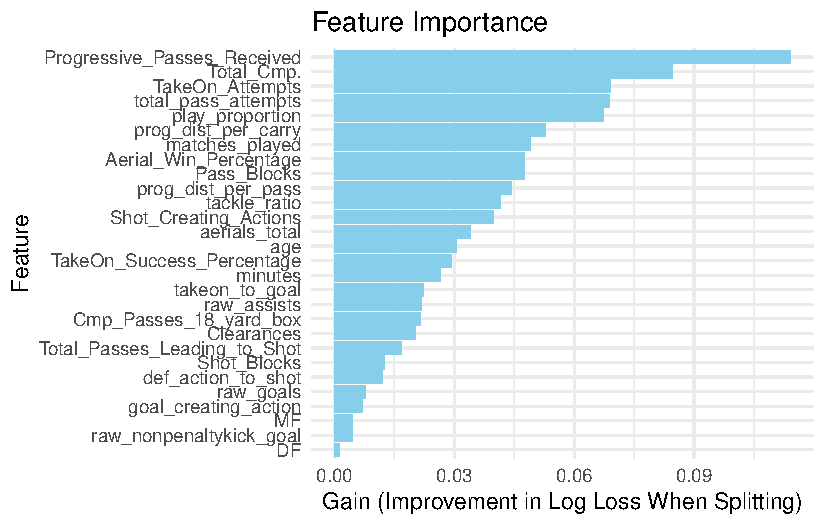
\includegraphics{aaron_lightGBM_modeling_files/figure-pdf/unnamed-chunk-13-1.pdf}

Save Plots

\begin{Shaded}
\begin{Highlighting}[]
\FunctionTok{ggsave}\NormalTok{(}\StringTok{"lightgbm\_roc.png"}\NormalTok{, }\AttributeTok{plot =}\NormalTok{ roc\_g, }\AttributeTok{width =} \DecValTok{8}\NormalTok{, }\AttributeTok{height =} \DecValTok{6}\NormalTok{)}
\FunctionTok{ggsave}\NormalTok{(}\StringTok{"lightgbm\_pr\_curve.png"}\NormalTok{, }\AttributeTok{plot =}\NormalTok{ pr\_curve\_g, }\AttributeTok{width =} \DecValTok{8}\NormalTok{, }\AttributeTok{height =} \DecValTok{6}\NormalTok{)}
\FunctionTok{ggsave}\NormalTok{(}\StringTok{"lightgbm\_conf\_matrix.png"}\NormalTok{, }\AttributeTok{plot =}\NormalTok{ conf\_matrix\_g, }\AttributeTok{width =} \DecValTok{8}\NormalTok{, }\AttributeTok{height =} \DecValTok{6}\NormalTok{)}
\FunctionTok{ggsave}\NormalTok{(}\StringTok{"lightgbm\_var\_import.png"}\NormalTok{, }\AttributeTok{plot =}\NormalTok{ variable\_importance\_g, }\AttributeTok{width =} \DecValTok{8}\NormalTok{, }
       \AttributeTok{height =} \DecValTok{6}\NormalTok{)}
\end{Highlighting}
\end{Shaded}





\end{document}
